\begin{surferPage}[D4--]{A $D_4^{--}$ Singularity}
The following equation corresponds to the so-called $D_4^{--}$-singularity:
    \vspace*{-0.4em}
    \begin{center}
      $x^2y-y^3-z^2=0.$
    \end{center}
    \vspace*{-0.4em}
    This is the surface variant of a plane singularity which 
    is a point in which three distinct straight lines meet.
    We get these three lines back from the surface equation when
    plugging $z=0$ into the equation.
    This yields the plane curve with equation $x^2y-y^3=0$ which is
    equivalent to $y\cdot(x-y)\cdot(x+y)=0$ (three straight lines, indeed):
    \vspace*{-0.7em}
    \begin{center}
      \begin{tabular}{c@{\ }c@{\ }c@{\ }c}
        \begin{tabular}{@{}c@{}}
          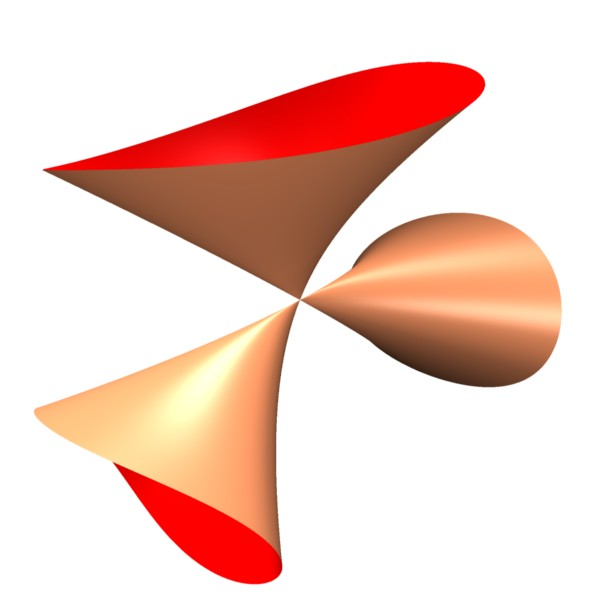
\includegraphics[width=1.2cm]{../../common/images/D4mm_0}
        \end{tabular}
        &
        \begin{tabular}{@{}c@{}}
          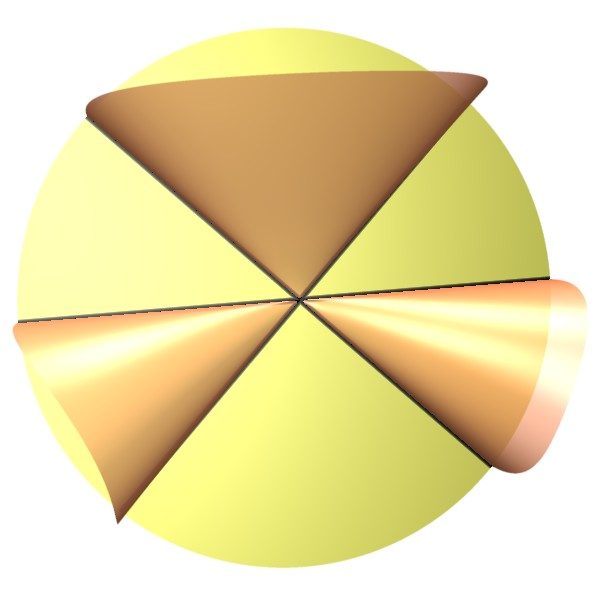
\includegraphics[width=1.2cm]{../../common/images/D4mm_def_with_plane_cut_0}
        \end{tabular}
     \end{tabular}
    \end{center}
    \vspace*{-0.4em}

    A good way to understand the geometry of this singularity 
is to look at a special kind of deformation of it:
The one where the singularity splits into three ordinary double points
($A_1$-singularities). 
Here, $a=0$ corresponds to the original equation:
\[(y+a)\cdot(x-y)\cdot(x+y)-z^2=0.\]
   \vspace*{-1em}
    \begin{center}
      \begin{tabular}{@{}c@{\quad}c@{\quad}c@{}}
        \begin{tabular}{@{}c@{}}
          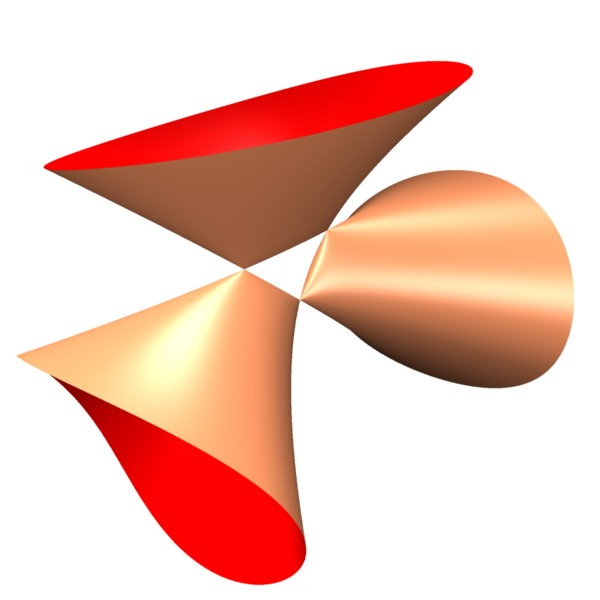
\includegraphics[width=1.1cm]{../../common/images/D4mm_1}
        \end{tabular}
        &
        \begin{tabular}{@{}c@{}}
          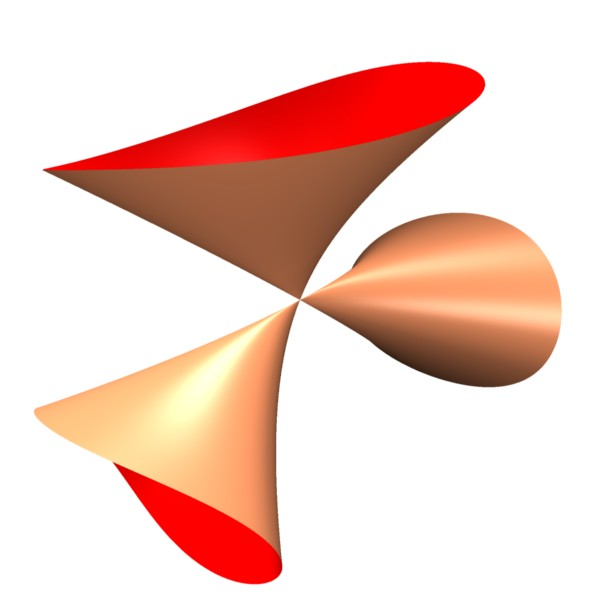
\includegraphics[width=1.1cm]{../../common/images/D4mm_0}
        \end{tabular}
        &
        \begin{tabular}{@{}c@{}}
          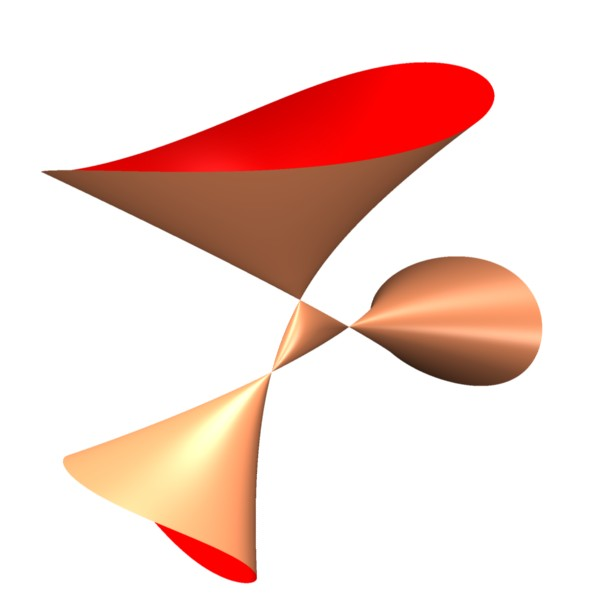
\includegraphics[width=1.1cm]{../../common/images/D4mm_2}
        \end{tabular}
\\
$a=-0.5$
& 
$a=0$
&
$a=0.5$
      \end{tabular}
    \end{center}
 
\end{surferPage}
